\documentclass[11pt]{standalone}
\usepackage{tikz}
\tikzset{
    B/.style={circle,draw=black,fill=blue,minimum size=5mm,inner sep=0mm},
    R/.style={circle,draw=black,fill=red,minimum size=5mm,inner sep=0mm},
    pics/necklace/.style n args={5}{
        code = {
            \begin{scope}
                \draw (0,0) node[#1]{} 
                    -- (0,2) node[#2]{} 
                    -- (2,2) node[#3]{}
                    -- (2,0) node[#4]{}
                    -- cycle;
                \node at (1,1) {\large\colorbox{#5}{$#1#2#3#4$}};
            \end{scope}
        }
    }
}
\begin{document}
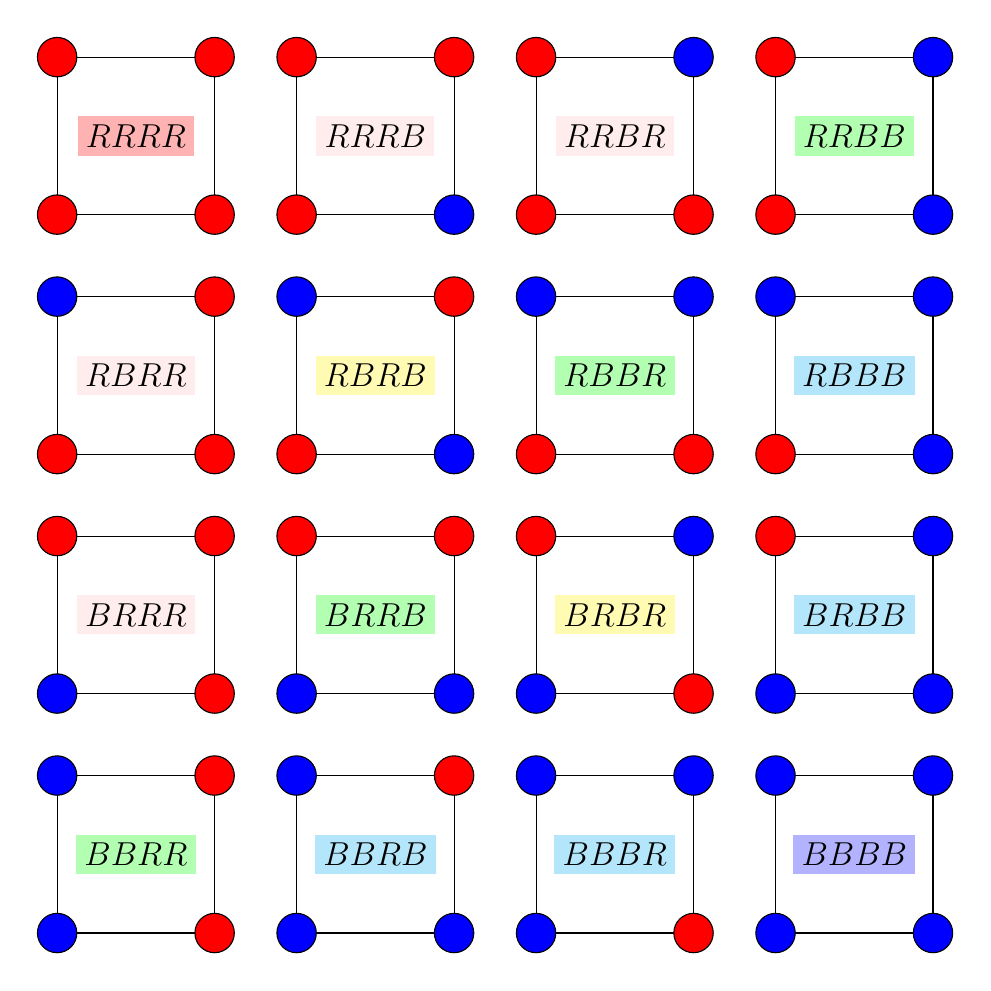
\begin{tikzpicture}
    \matrix [column sep=1.5em, row sep=1.5em, cells={draw}] {
        \pic {necklace={R}{R}{R}{R}{red!30}};  &
        \pic {necklace={R}{R}{R}{B}{pink!30}};  &
        \pic {necklace={R}{R}{B}{R}{pink!30}};  &
        \pic {necklace={R}{R}{B}{B}{green!30}};
        \\
        \pic {necklace={R}{B}{R}{R}{pink!30}};  &
        \pic {necklace={R}{B}{R}{B}{yellow!30}};  &
        \pic {necklace={R}{B}{B}{R}{green!30}};  &
        \pic {necklace={R}{B}{B}{B}{cyan!30}};
        \\
        \pic {necklace={B}{R}{R}{R}{pink!30}};  &
        \pic {necklace={B}{R}{R}{B}{green!30}};  &
        \pic {necklace={B}{R}{B}{R}{yellow!30}};  &
        \pic {necklace={B}{R}{B}{B}{cyan!30}};
        \\
        \pic {necklace={B}{B}{R}{R}{green!30}};  &
        \pic {necklace={B}{B}{R}{B}{cyan!30}};  &
        \pic {necklace={B}{B}{B}{R}{cyan!30}};  &
        \pic {necklace={B}{B}{B}{B}{blue!30}};
        \\
    };
\end{tikzpicture}
\end{document}​
